\subsubsection{Disadvantages of the text comparison function}

The first disadvantage of the text comparison function was maybe the restriction of the length of a phrase. By default a phrase was a list of tokens which was more than 4 tokens. That means it could be difficult to find out plagiarized positions if their length was less than 4 tokens. 

Another disadvantage was that the strict comparison algorithm could compare only continual phrases. That means if at some positions there was a tiny change such as a break line or a comma, the algorithm could miss them.

\begin{figure}[!h]
  \centering
  \fbox{
    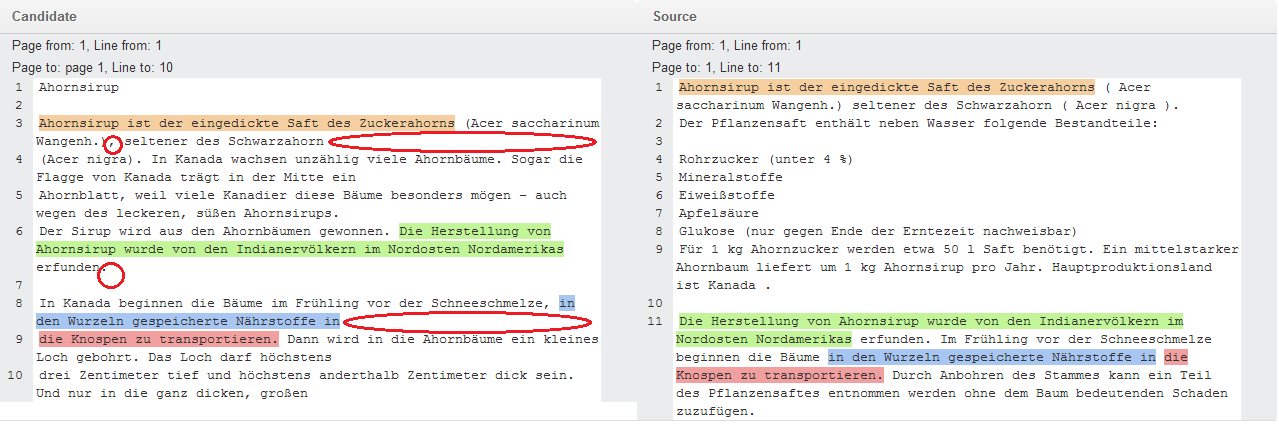
\includegraphics[width=0.97\textwidth]{images/strict_algo.png}
  }
  \caption{a strict comparison algorithm}
  \label{fig:report_deckblatt}
\end{figure}

Here is the source code of compare text function

\begin{lstlisting}[caption=Cropping an image to a square aspect ratio]
private static function compareText($documents, $min_run_length){
    $documents_len = array();

    $final_match_list = array();
    $match_table = array();
    $docs = sizeof($documents);

    for($doc_idx = 0; $doc_idx < $docs; $doc_idx++){
      $doc = $documents[$doc_idx];
      $tokens = sizeof($doc) - $min_run_length + 1;
      $doc_len = sizeof($doc);
      $documents_len[$doc_idx] = $doc_len;

      // If the word is smaller than the min_run_length, do not analyse it
      if($tokens <= 0){
        continue;
      }

      $min_token_idx = 0;

      for($token_idx = 0; $token_idx < $tokens; $token_idx++){
        $match = array_slice($doc, $token_idx, $min_run_length);
        $match_loc = array($doc_idx, $token_idx);
        $match_tag = implode(" ", $match);

        if(array_key_exists($match_tag, $match_table)){
          if($token_idx >= $min_token_idx){
            $best_match = array($doc_idx, $token_idx, -1, 0, 0);
            $matches = $match_table[$match_tag];
            $nr_matches = sizeof($matches);
            for($idx = 0; $idx < $nr_matches; $idx++){
              $match_peer = $matches[$idx];
              $peer_doc_idx = $match_peer[0];
              $peer_doc = $documents[$peer_doc_idx];
              $peer_token_idx = $match_peer[1] + $min_run_length;
              $peer_len = $documents_len[$peer_doc_idx];
              $our_token_idx = $token_idx + $min_run_length;

              if($peer_doc_idx == $doc_idx){
                continue;
              }

              while($peer_token_idx < $peer_len
              && $our_token_idx < $doc_len
              && $peer_doc[$peer_token_idx] == $doc[$our_token_idx]){
                $peer_token_idx++;
                $our_token_idx++;
              }

              $len = $our_token_idx - $token_idx;
              if($len > $best_match[4]){
                $best_match[2] = $match_peer[0];
                $best_match[3] = $match_peer[1];
                $best_match[4] = $len;
              }
            }

            if($best_match[2] != -1){
              array_push($final_match_list, $best_match);
              $min_token_idx = $token_idx + $best_match[4];
            }
          }
          array_push($match_table[$match_tag], $match_loc);
        }else{
          $match_table[$match_tag] = array($match_loc);
        }
      }
    }
    return $final_match_list;
  }
\end{lstlisting}